% 2011 年浙江卷文科第 10 题：四个 y=f(x) 图象选项。
% 来源 PDF：普通高考/2011/2011浙江文.pdf，SHA-256 36931500dfd850579d93f0a685f0ccea25065c84c09db5157c451093d53b56f0。
% 原页：第 1 页第 2 栏，书页码 711。示意图；x=-1 用虚线标出。
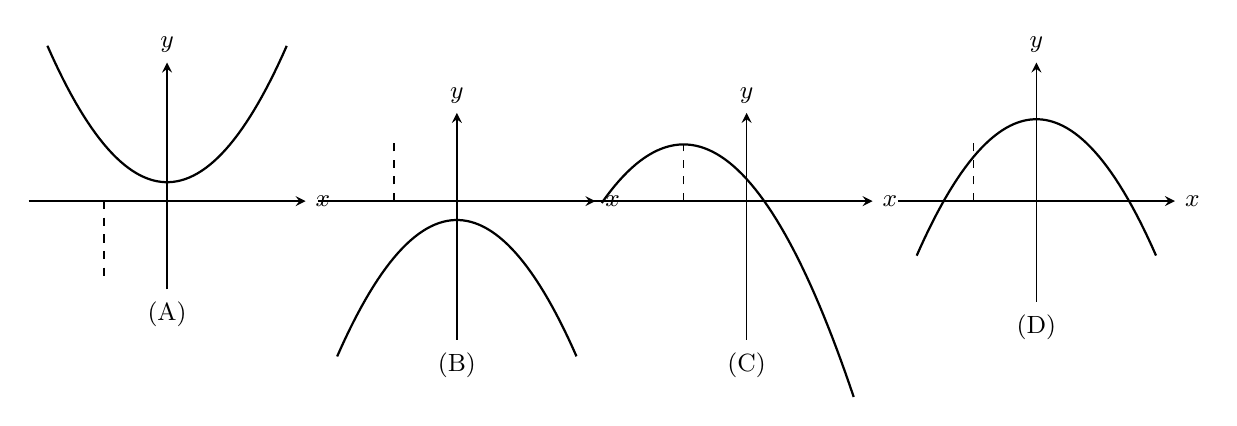
\begin{tikzpicture}[>=stealth, semithick, font=\small, scale=0.8]
  % (A) 开口向上，截距正
  \begin{scope}
    \draw[->] (-2.2,0)--(2.2,0) node[right] {$x$};
    \draw[->] (0,-1.4)--(0,2.2) node[above] {$y$};
    \draw[dashed] (-1,0)--(-1,-1.2);
    \draw[thick, domain=-1.9:1.9, samples=60] plot (\x,{0.6*\x*\x+0.3});
    \node at (0,-1.8) {(A)};
  \end{scope}
  % (B) 开口向下，截距负
  \begin{scope}[xshift=4.6cm]
    \draw[->] (-2.2,0)--(2.2,0) node[right] {$x$};
    \draw[->] (0,-2.2)--(0,1.4) node[above] {$y$};
    \draw[dashed] (-1,0)--(-1,1.0);
    \draw[thick, domain=-1.9:1.9, samples=60] plot (\x,{-0.6*\x*\x-0.3});
    \node at (0,-2.6) {(B)};
  \end{scope}
  % (C) 开口向下，顶点在 x=-1 附近，截距负
  \begin{scope}[xshift=9.2cm]
    \draw[->] (-2.6,0)--(2.0,0) node[right] {$x$};
    \draw[->] (0,-2.2)--(0,1.4) node[above] {$y$};
    \draw[dashed] (-1,0)--(-1,0.9);
    \draw[thick, domain=-2.3:1.7, samples=60] plot (\x,{-0.55*(\x+1)*(\x+1)+0.9});
    \node at (0,-2.6) {(C)};
  \end{scope}
  % (D) 开口向下，但截距为正（不可能）
  \begin{scope}[xshift=13.8cm]
    \draw[->] (-2.2,0)--(2.2,0) node[right] {$x$};
    \draw[->] (0,-1.6)--(0,2.2) node[above] {$y$};
    \draw[dashed] (-1,0)--(-1,1.0);
    \draw[thick, domain=-1.9:1.9, samples=60] plot (\x,{-0.6*\x*\x+1.3});
    \node at (0,-2.0) {(D)};
  \end{scope}
\end{tikzpicture}
